\chapter{Analisi preliminare}

Nel presente capitolo viene descritta l’analisi preliminare svolta a monte dello sviluppo del sistema. Essa ha riguardato la definizione del problema, l’individuazione degli obiettivi e la suddivisione di ruoli e attività tra i membri del gruppo.

\section{Ruoli e gestione del gruppo}

Il team di progetto è eterogeneo ed è composto da quattro studenti, due provenienti da Ingegneria Informatica e due da Ingegneria Gestionale. In generale, la separazione dei ruoli non è stata vincolante, ma ha favorito la collaborazione continua tra i due team mediante contaminazioni costruttive.

I membri di area gestionale si sono occupati principalmente della pianificazione temporale del progetto, articolando le macro-attività e le relative sotto-attività attraverso un diagramma di Gantt. Tale fase è stata supportata da una \textit{Work Breakdown Structure} (WBS), utilizzata per scomporre il progetto in fasi dettagliate e sequenziali, organizzando le attività in modo progressivo.

Gli studenti di area informatica si sono invece occupati della progettazione e dello sviluppo del sistema. In particolare, il lavoro ha riguardato l’analisi dei requisiti funzionali e non funzionali, il \textit{benchmarking} tecnologico, la progettazione dell’architettura, l’implementazione di tutti i moduli software e la fase finale di test e deployment del prototipo.

Nella prima fase, il team gestionale ha partecipato al recupero delle informazioni dalle fonti ufficiali dei Giochi del Mediterraneo e da fonti terze online per la costruzione della knowledge base. Successivamente, il lavoro sui dati è proseguito con la pulizia e il preprocessing dei contenuti testuali fino alla conversione in record strutturati in formato \textit{JSONL}.

In seguito, il team informatico ha svolto la fase di benchmarking tecnologico mediante un'analisi comparativa di diverse soluzioni open-source e commerciali per il retrieval semantico, la generazione di testo e l'integrazione con modelli linguistici di grandi dimensioni (LLM) con l'obiettivo di individuare il compromesso ottimale tra performance, flessibilità e sostenibilità economica per la scelta delle tecnologie da adottare nel progetto. Il team gestionale ha contribuito a tale fase, supportando la valutazione dal punto di vista della compatibilità con gli obiettivi del progetto, dei costi e della coerenza con il valore di business della soluzione.

Nell’ultima fase di test, il lavoro sinergico tra il team gestionale e il team informatico ha permesso di ottenere risultati concreti e misurabili per la valutazione complessiva del sistema. Il team gestionale ha contribuito alla costruzione di un dataset di test il più possibile vicino a potenziali interazioni reali degli utenti, mentre il team informatico ha sviluppato lo script di automazione necessario per eseguire i test e raccogliere le metriche di valutazione.

Trasversalmente a tutte le fasi di progetto, il team gestionale ha avuto il compito di organizzare le riunioni settimanali con i tutor aziendali e di monitorare l’avanzamento rispetto alle scadenze previste nel Gantt, mentre il team informatico ha prodotto i deliverables tecnici e le presentazioni per le riunioni intermedie.

Per la gestione delle attività è stato utilizzato Trello come bacheca principale, secondo un'organizzazione Agile semplificata con \textit{Kanban board}. L'adozione di un approccio Kanban si è rivelata particolarmente efficace per la gestione di un progetto dalla durata contenuta, consentendo al team di mantenere alta la visibilità sullo stato di avanzamento, di identificare tempestivamente eventuali blocchi e di ripianificare le priorità in modo dinamico, senza gli overhead tipici di metodologie più rigorose come Scrum. In Figura~\ref{fig:trello-board} è riportata una schermata della bacheca.

\begin{figure}[H]
\centering
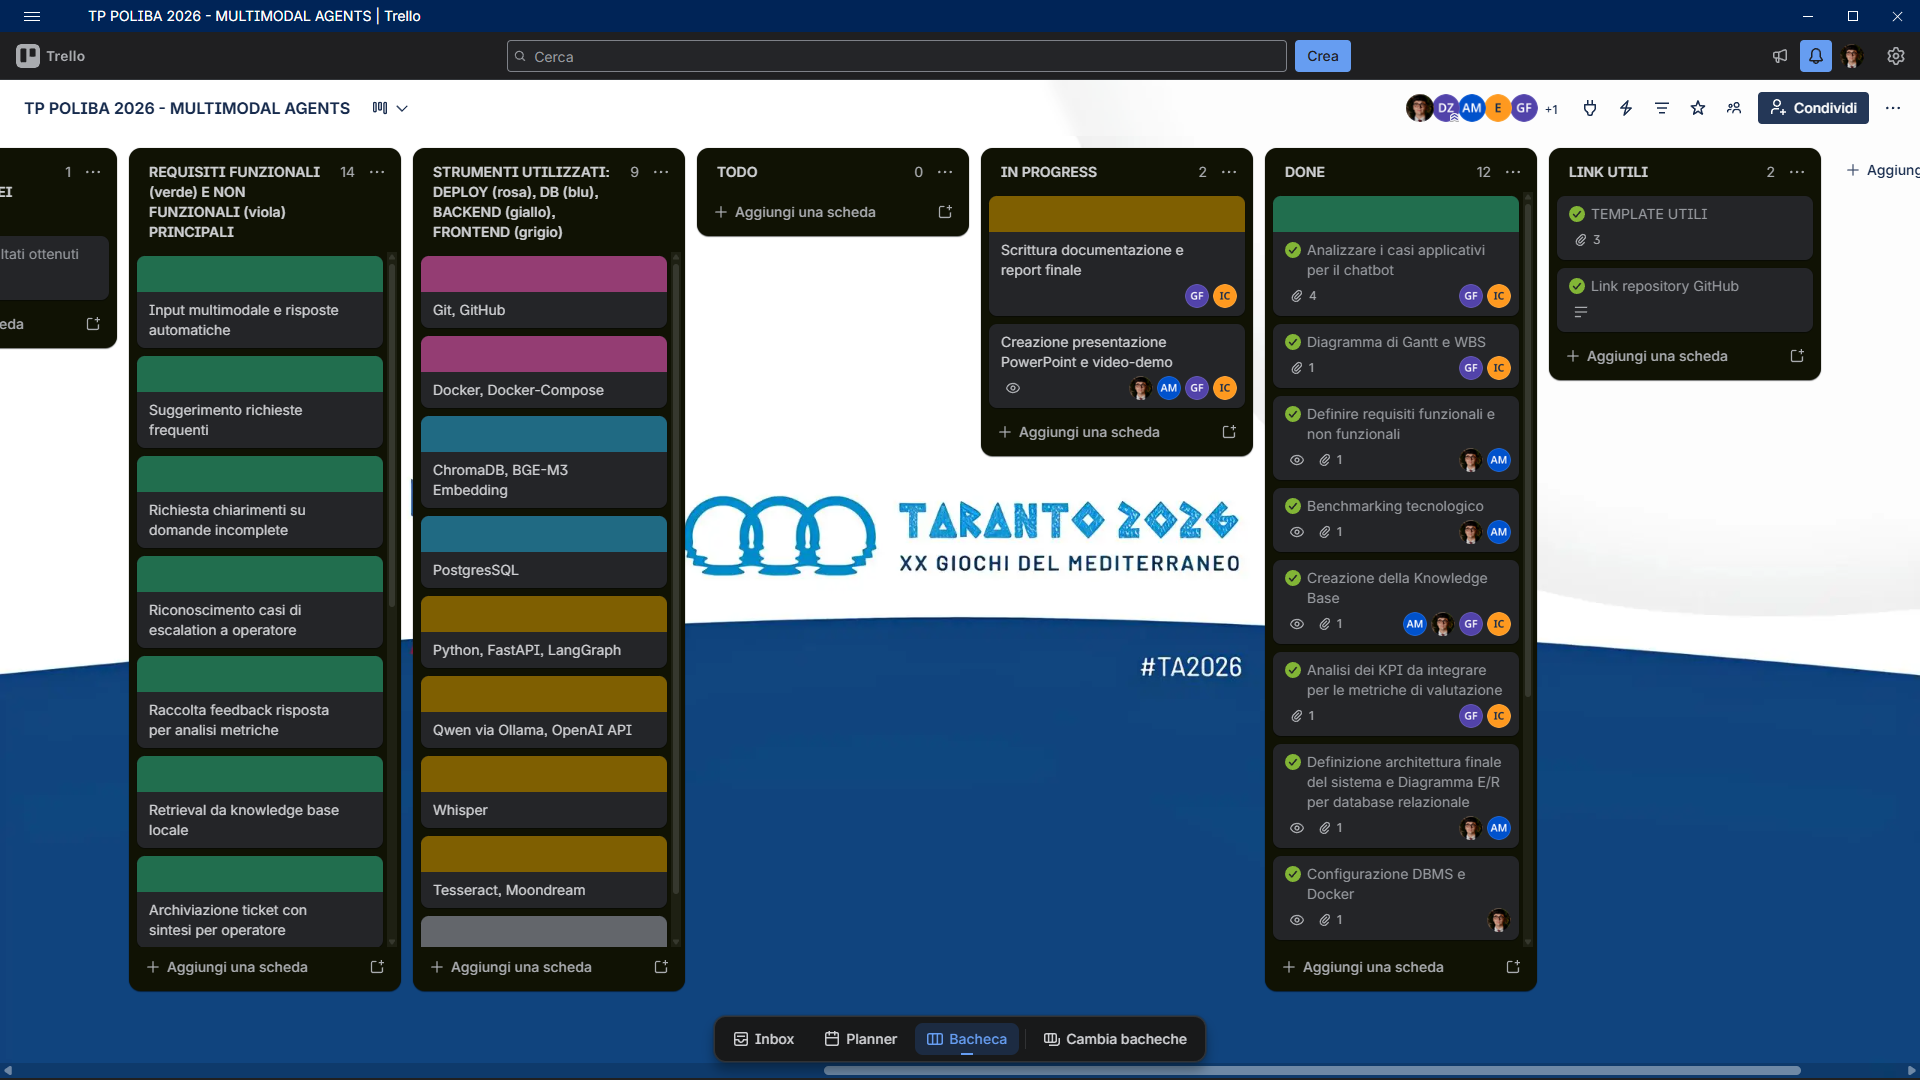
\includegraphics[width=0.95\textwidth]{images/trello-screen.png}
\caption{Bacheca Trello utilizzata per l’organizzazione delle attività di progetto.}\label{fig:trello-board}
\end{figure}

Inoltre, come canali di comunicazione sono stati utilizzati Slack e Microsoft Teams. Il primo ha rappresentato il mezzo principale per interfacciarsi con i tutor aziendali, mentre il secondo è stato utilizzato per le riunioni da remoto e per lo scambio di messaggi e materiale tra i componenti del team. Le principali sfide incontrate hanno riguardato l'integrazione tra le due componenti del team, sia in termini di allineamento terminologico (linguaggio tecnico vs manageriale), sia nella definizione di interfacce chiare tra il lavoro di preparazione dei dati e quello di sviluppo software. Tali difficoltà sono state, però, superate attraverso le riunioni di allineamento frequenti e la creazione di artefatti condivisi (documenti di specifica, dizionario dei dati, repository comune), rafforzando la coesione del gruppo e la qualità complessiva del risultato finale.

\section{Diagramma di Gantt e Work Breakdown Structure}

Il diagramma di Gantt ha avuto lo scopo di distribuire le attività nel tempo e tra le risorse. La WBS, invece, ha permesso di scomporre il progetto in fasi e sotto-attività. Il periodo di lavoro è stato organizzato su un intervallo di circa due mesi, mentre la pianificazione è stata articolata in settimane. Il Gantt sintetico, mostrato in Figura~\ref{fig:gantt-sintesi}, riassume le principali macro-attività svolte dal team, mentre il Gantt dettagliato, mostrato in Figura~\ref{fig:gantt-dettaglio}, esplicita anche le singole sotto-attività, i responsabili e le risorse di supporto.

\begin{figure}[H]
\centering
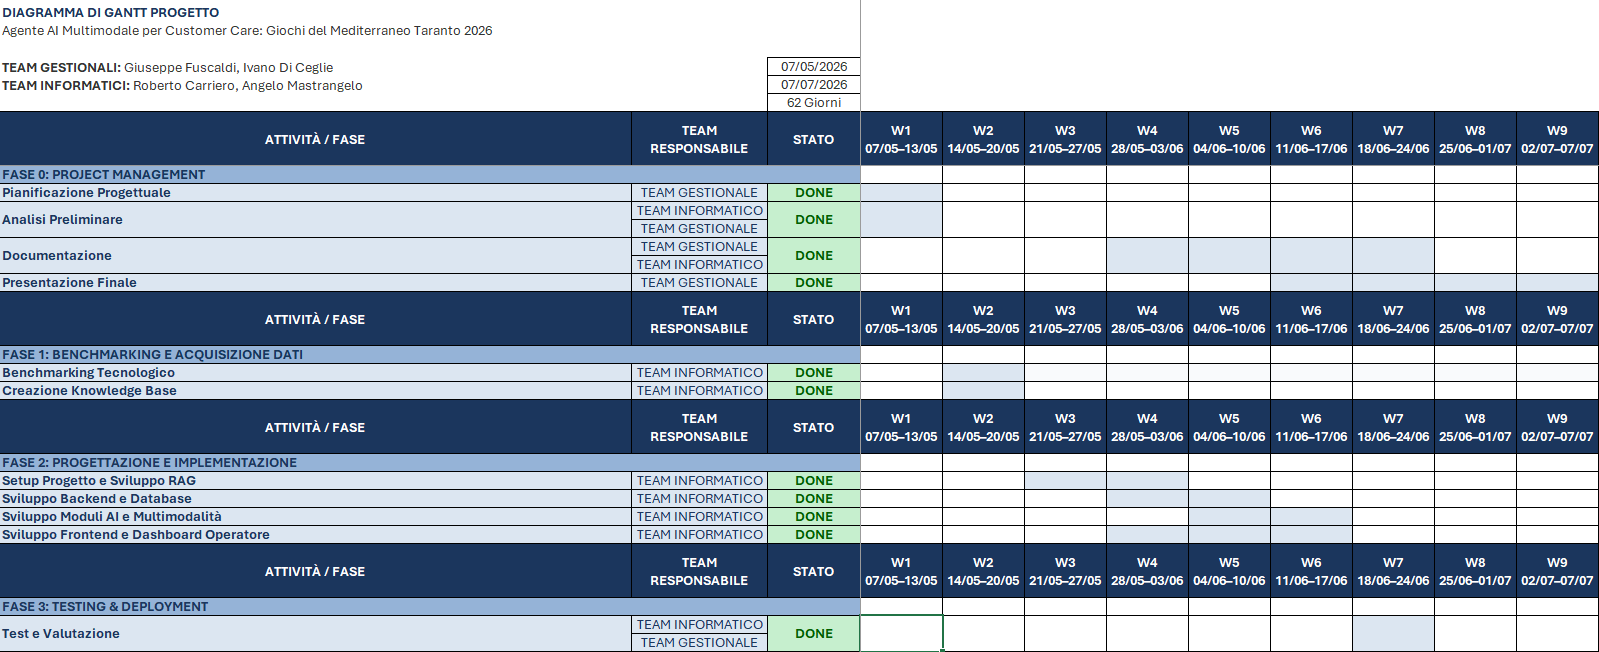
\includegraphics[width=0.95\textwidth]{images/gantt-sintesi.png}
\caption{Rappresentazione sintetica del diagramma di Gantt del progetto.}\label{fig:gantt-sintesi}
\end{figure}

\begin{figure}[H]
\centering
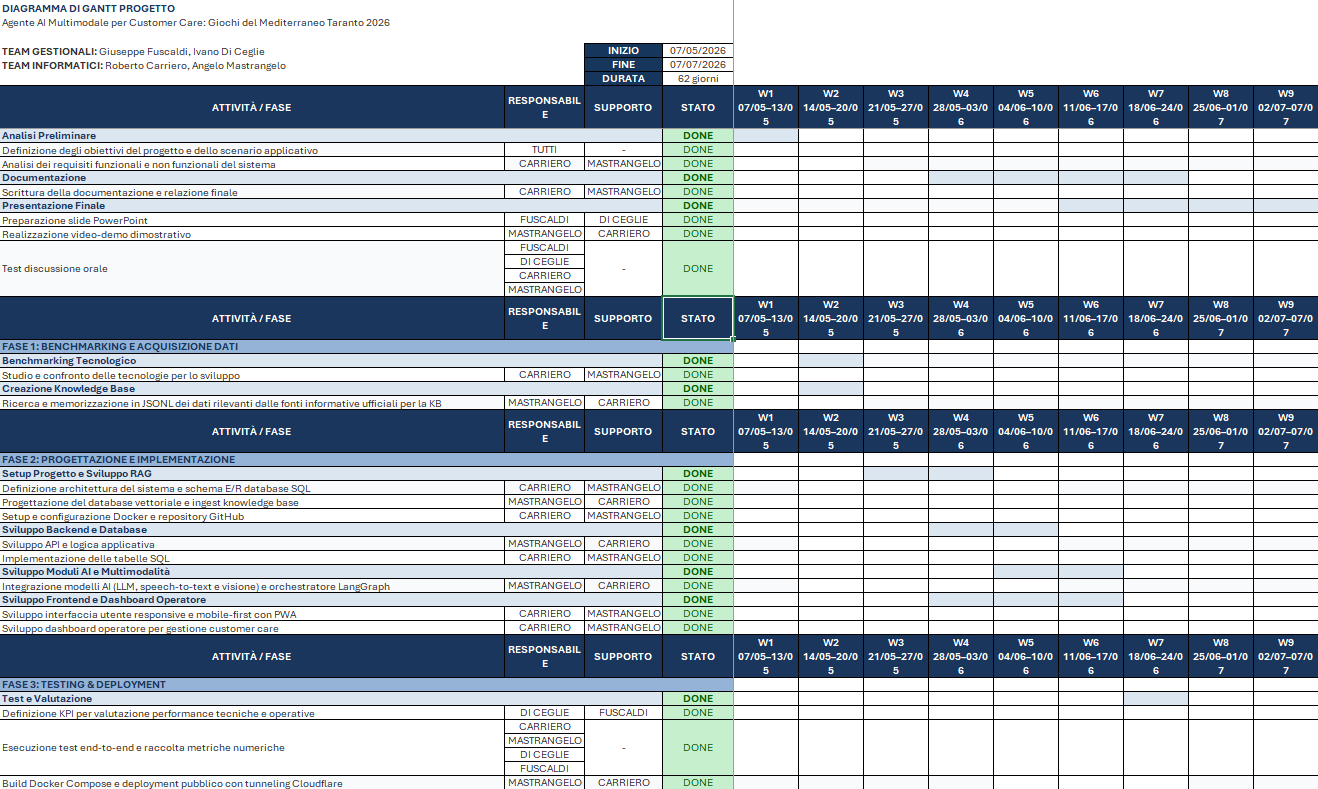
\includegraphics[width=0.95\textwidth]{images/gantt-dettagli.png}
\caption{Rappresentazione dettagliata del diagramma di Gantt con attività, responsabili e avanzamento.}\label{fig:gantt-dettaglio}
\end{figure}

Dal punto di vista organizzativo, il progetto è stato suddiviso in quattro aree. La prima area riguarda il project management e le attività trasversali, la seconda area include il benchmarking e l’acquisizione dei dati, la terza area comprende la progettazione e l’implementazione del sistema, mentre la quarta area integra il testing e il deployment del sistema.

\section{Requisiti funzionali e non funzionali}

La definizione dei requisiti ha anticipato la progettazione del sistema. In generale, per lo sviluppo di una soluzione software è necessario chiarire quali funzionalità essa deve offrire e quali qualità deve garantire.

I requisiti funzionali descrivono le caratteristiche del sistema. Nel caso specifico, il chatbot deve consentire all’utente di formulare richieste in linguaggio naturale e di interagire attraverso formati di input diversi. Tali input devono essere ricondotti a una rappresentazione interna coerente, così da poter essere elaborati dalla stessa pipeline applicativa. Il sistema deve poi recuperare le informazioni rilevanti dalla base di conoscenza, generare risposte automatiche coerenti e aiutare l’utente nell’escalation in caso di insoddisfazione.

Il sistema deve inoltre memorizzare conversazioni, messaggi, feedback e ticket in una base di dati per poterli analizzare successivamente. La raccolta dei feedback è prioritaria, in quanto consente di valutare la qualità percepita della risposta e la soddisfazione dell'utente, mentre la dashboard di customer care rappresenta il principale punto di contatto tra l'utente e l'operatore umano.

Accanto ai requisiti funzionali sono stati definiti i requisiti non funzionali, letti secondo il modello \textit{Functionality, Usability, Reliability, Performance, Supportability +} (FURPS+), come descritto di seguito.

Dal punto di vista della funzionalità \textit{(F)}, il sistema deve interpretare correttamente le richieste, distinguere tra risposta automatica ed escalation e ridurre il rischio di risposte non supportate da fonti certe.
Dal punto di vista dell’usabilità \textit{(U)}, l’interfaccia deve essere semplice e accessibile da diversi dispositivi. Per l’affidabilità \textit{(R)}, il chatbot deve poter gestire input incompleti o poco chiari, privilegiando il chiarimento o il passaggio all’operatore invece di generare informazioni non verificate.
In riferimento alle prestazioni \textit{(P)}, il sistema deve mantenere tempi di risposta compatibili con una conversazione umana, nonostante la complessità della pipeline.
Dal punto di vista della supportabilità \textit{(S)}, l’architettura deve essere modulare, testabile e scalabile. La base di conoscenza deve poter essere aggiornata senza riprogettare il sistema, mentre la containerizzazione deve rendere l’ambiente replicabile su macchine diverse.
Un requisito trasversale è la tracciabilità \textit{(+)}, poiché ogni risposta deve riportare esplicitamente le fonti consultate per garantire l'attendibilità delle risposte automatiche.

\section{Denominazione e branding}

Per il nome del sistema è stato scelto l’acronimo T.A.L.O.S. \textit{(Taranto 2026 AI Live Operator Support)}. Il nome richiama Talos, figura della mitologia greca descritta come un gigante di bronzo creato da Efesto per proteggere l’isola di Creta. Questo riferimento si sposa bene con le radici storiche e culturali della Magna Grecia, a cui Taranto è profondamente legata, e con l’idea di un sistema intelligente posto a supporto degli utenti.

Per il branding è stata scelta una comunicazione visuale coerente con il contesto dei Giochi del Mediterraneo, ma allo stesso tempo riconoscibile e personalizzata rispetto al progetto. Dunque, il logo del sistema riprende Ionios, la mascotte di Taranto 2026, reinterpretandola in chiave customer care. Infatti, sul capo della mascotte è stata aggiunta una cuffia da operatore e sul petto il logo di TP, come mostrato in Figura~\ref{fig:talos-mascot}.

\begin{figure}[H]
\centering

\includegraphics[width=0.4\textwidth]{images/talos_mascot.png}
\caption{Logo del sistema T.A.L.O.S.}\label{fig:talos-mascot}
\end{figure}

\section{Creazione della knowledge base}

La creazione della knowledge base rappresenta una delle fasi più delicate del progetto, poiché la qualità delle risposte del chatbot dipende direttamente dalla qualità delle informazioni disponibili.

La prima fase ha riguardato il recupero manuale delle informazioni da fonti diverse. La principale fonte è stata il sito ufficiale dei Giochi del Mediterraneo Taranto 2026\footnote{\url{https://www.ta2026.com/}}, utilizzato per raccogliere dati relativi all’evento, alle discipline sportive e alle sedi di gara. A tale fonte sono state affiancate pagine secondarie, tra cui Wikipedia\footnote{\url{https://it.wikipedia.org/wiki/Giochi_del_Mediterraneo}}, per il contesto storico generale, e il sito ufficiale del Comitato Internazionale dei Giochi del Mediterraneo, CIJM\footnote{\url{https://cijm.org.gr/}}, per informazioni relative alle edizioni precedenti e al contesto istituzionale della manifestazione.

Dopo la fase di recupero delle informazioni, è stato necessario attuare una fase di pulizia e normalizzazione del materiale per rimuovere le impurità tipiche delle fonti web, come residui HTML, link duplicati e contenuti ridondanti o irrilevanti.

La knowledge base finale è stata salvata in formato JSONL, cioè JSON Lines. In questo formato, ogni riga del file rappresenta un record \textit{JSON} indipendente, facile da caricare e indicizzare nel database vettoriale per il RAG. Ogni record della knowledge base è composto da tre elementi principali, ovvero \textit{id}, \textit{document} e \textit{metadata}, come riassunto in Tabella \ref{tab:kb-record-structure}.

\begin{table}[H]
\centering
\renewcommand{\arraystretch}{1.25}
\begin{tabular}{p{0.30\textwidth} p{0.60\textwidth}}
\toprule
\textbf{Campo} & \textbf{Descrizione} \\
\midrule
\textbf{id}& Identificativo univoco del record, utile per distinguere ogni informazione all’interno della knowledge base. \\
\textbf{document}& Testo discorsivo contenente l’informazione da indicizzare e recuperare tramite ricerca semantica. \\
\textbf{metadata.type}& Tipologia del contenuto, ad esempio venue, sport, calendario, ticketing, contatto, informazione storica o contenuto istituzionale. \\
\textbf{metadata.title}& Titolo sintetico del record, utile per riconoscere rapidamente il contenuto recuperato. \\
\textbf{metadata.source\_url}& Collegamento alla fonte da cui deriva l’informazione, usato per garantire tracciabilità. \\
\textbf{metadata.address}& Indirizzo del luogo, presente quando il record riguarda una sede fisica o una venue. \\
\textbf{metadata.latitude}, \textbf{metadata.longitude}& Coordinate geografiche, presenti quando disponibili, utilizzabili per generare collegamenti a servizi di navigazione. \\
\bottomrule
\end{tabular}
\caption{Struttura logica dei record della knowledge base.}\label{tab:kb-record-structure}
\end{table}

La knowledge base contiene \textit{2557} record distinti, riguardanti tutti gli aspetti principali dell'evento.

In particolare, per i record relativi alle \textit{venue}, ovvero ai luoghi di gioco, sono stati inseriti indirizzi e coordinate geografiche oltre a caratteristiche di accessibilità, come parcheggi e trasporti pubblici. I record relativi al calendario delle gare contengono informazioni su date, fasi e associazioni tra sport e sedi nelle città coinvolte. Sono presenti, inoltre, record storici di repertorio relativi alle edizioni passate con riferimento alle nazioni e agli atleti partecipanti, nonché alle migliori prestazioni ottenute.

Per il ticketing, poiché al momento della costruzione della knowledge base non risultavano pubblicate informazioni ufficiali sufficientemente dettagliate, è stato creato un record specifico che segnala l’assenza del dato. In questo modo, il chatbot può rispondere in modo prudente, evitando di generare informazioni false e mantenendosi entro un guardrail informativo.

Le fasi di creazione della base di conoscenza sono riassunte in Tabella \ref{tab:kb-pipeline}.

\begin{table}[H]
\centering
\renewcommand{\arraystretch}{1.25}
\begin{tabular}{p{0.25\textwidth} p{0.62\textwidth}}
\toprule
\textbf{Fase} & \textbf{Descrizione} \\
\midrule
\textbf{Raccolta fonti} & Recupero manuale di informazioni da sito ufficiale Taranto 2026, CIJM, Wikipedia e altre fonti online. \\
\textbf{Selezione contenuti} & Individuazione delle informazioni utili per le risposte. \\
\textbf{Pulizia} & Rimozione di residui HTML, contenuti ripetuti e porzioni testuali non utili al retrieval. \\
\textbf{Normalizzazione} & Riscrittura dei contenuti in forma discorsiva e con traduzione uniforme. \\
\textbf{Strutturazione} & Conversione delle informazioni in record \textit{JSONL} composti da \textit{id}, \textit{document} e \textit{metadata}. \\
\textbf{Validazione} & Controllo di duplicati, record vuoti, fonti mancanti e metadati incompatibili con l’ingest. \\
\textbf{Ingest} & Indicizzazione dei record nel database vettoriale per consentire il retrieval semantico. \\
\bottomrule
\end{tabular}
\caption{Fasi principali di costruzione della knowledge base.}\label{tab:kb-pipeline}
\end{table}

\section{Benchmarking tecnologico}

Il benchmarking tecnologico è stato svolto per individuare le soluzioni più adatte da integrare nello sviluppo del sistema. Le metriche principali utilizzate per il confronto sono state quattro: il costo, inteso sia come eventuale costo di licenza o utilizzo di servizi esterni, sia come costo indiretto legato alle risorse computazionali richieste, la semplicità di utilizzo, collegata alla curva di apprendimento e alla rapidità con cui la tecnologia può essere adottata in un project work con tempi limitati, facilità di integrazione con il resto dello stack applicativo e la disponibilità di documentazione, considerata rilevante per ridurre il rischio di blocchi tecnici durante lo sviluppo.

\subsection*{Frontend}

Il frontend è la parte dell’applicazione con cui l’utente interagisce direttamente. Nel progetto comprende la chat pubblica, la dashboard dell’operatore e la pagina per la gestione della knowledge base. La scelta della tecnologia frontend era quindi importante per garantire un’interfaccia responsive, utilizzabile da dispositivi diversi e abbastanza flessibile da supportare più pagine e componenti.

Per questa componente sono state considerate soluzioni come React, Streamlit e Gradio. React è una libreria JavaScript per la costruzione di interfacce utente basate su componenti riutilizzabili. Streamlit è un framework Python pensato per creare rapidamente interfacce web, soprattutto per applicazioni data science e prototipi AI. Gradio è uno strumento orientato alla creazione veloce di demo per modelli di machine learning e intelligenza artificiale.

Dal punto di vista del costo, tutte le soluzioni sono risultate favorevoli, poiché utilizzabili senza costi diretti nel contesto del progetto. Streamlit e Gradio sono molto semplici da usare e presentano una curva di apprendimento ridotta, ma risultano meno adatti alla costruzione di una piattaforma web completa, con gestione dello stato, routing tra pagine, componenti personalizzati, interfacce responsive e separazione tra utente, operatore e amministratore. React richiede una maggiore configurazione iniziale, ma offre più controllo sull’interfaccia e una migliore scalabilità del frontend. Per questo motivo è stato scelto React, supportato da Vite per velocizzare lo sviluppo e da Tailwind CSS per gestire lo stile dell’interfaccia in modo modulare.

\subsection*{Backend}

Il backend è la componente server-side del sistema. Ha il compito di ricevere le richieste dal frontend, esporre gli endpoint API, coordinare la logica applicativa, interagire con i database e richiamare i moduli di intelligenza artificiale. Esso coordina la pipeline RAG, l’elaborazione multimodale, la generazione della risposta e l’eventuale apertura di ticket.

Per questa componente sono stati confrontati FastAPI, Flask e Django. FastAPI è un framework Python moderno per lo sviluppo di API web, con supporto alla validazione automatica dei dati e alla documentazione OpenAPI. Flask è un framework Python leggero e flessibile, adatto a servizi web semplici e personalizzabili. Django è un framework Python più completo e strutturato, che include molte funzionalità integrate, come gestione utenti, ORM e pannello amministrativo.

Dal punto di vista del costo, tutte le alternative sono open-source. La scelta è stata quindi guidata soprattutto da facilità di integrazione, documentazione e coerenza con una pipeline AI basata su Python. Flask è semplice, ma richiede maggiore lavoro manuale per validazione, organizzazione del progetto e documentazione degli endpoint. Django offre molte funzionalità, ma risulta più pesante rispetto alle esigenze di un backend AI multimodale. FastAPI rappresenta il miglior compromesso, perché consente di costruire API moderne, veloci, documentate automaticamente e facilmente integrabili con moduli Python specifici.

\subsection*{Database relazionale}

Il database relazionale è necessario per memorizzare i dati strutturati generati durante l’uso dell’applicazione. Nel progetto vengono salvati elementi come conversazioni, messaggi, feedback, ticket, operatori e dati collegati alle sessioni utente. Questi dati hanno relazioni precise tra loro e devono essere conservati in modo persistente.

Sono state considerate soluzioni come SQLite, MySQL e PostgreSQL. SQLite è un database relazionale leggero, basato su file, molto semplice da configurare e adatto a prototipi locali. MySQL è un sistema di gestione di database relazionali molto diffuso in ambito web. PostgreSQL è un database relazionale avanzato e robusto, adatto alla gestione di dati strutturati, relazioni complesse e applicazioni server-side.

Dal punto di vista del costo, tutte le soluzioni sono favorevoli. SQLite è il più semplice da utilizzare, ma risulta meno adatto a un sistema composto da più servizi containerizzati. MySQL rappresenta una soluzione valida e consolidata, ma PostgreSQL è stato preferito per robustezza, diffusione, stabilità e buona integrazione con backend moderni. Inoltre, PostgreSQL consente di separare chiaramente i dati operativi dal retrieval semantico, che viene invece gestito dal database vettoriale. Per facilitare la visualizzazione e la manutenzione delle tabelle è stato previsto anche pgAdmin, uno strumento grafico per amministrare database PostgreSQL.

\subsection*{Knowledge base}

La knowledge base è l’insieme strutturato delle informazioni da cui il sistema recupera i contenuti necessari per generare risposte. Nel progetto rappresenta una componente centrale, perché il chatbot deve rispondere utilizzando esclusivamente informazioni controllate e tracciabili.

Per strutturare la knowledge base sono state considerate alternative come CSV, documenti testuali non strutturati e JSONL. Il CSV è un formato tabellare semplice, utile quando i dati sono organizzati in righe e colonne regolari. I documenti testuali non strutturati sono file liberi, facili da creare ma più difficili da controllare durante l’indicizzazione. JSONL, cioè JSON Lines, è un formato in cui ogni riga rappresenta un oggetto JSON indipendente.

Il CSV è semplice e poco costoso, ma risulta meno flessibile quando ogni record deve contenere testo discorsivo e numerosi metadati. I documenti testuali non strutturati sono rapidi da produrre, ma rendono più complesso il controllo puntuale dei record. JSONL è stato scelto perché permette di rappresentare ogni informazione come un record autonomo, composto da contenuto testuale e metadati.

\subsection*{Embedding}

Gli embedding sono rappresentazioni numeriche di testi, domande o documenti. Servono a trasformare il linguaggio naturale in vettori, cioè insiemi di valori numerici che possono essere confrontati tra loro. Nella pipeline RAG, gli embedding permettono di confrontare la domanda dell’utente con i record della knowledge base e recuperare i documenti semanticamente più vicini.

Per questa componente sono state valutate soluzioni multilingua come BAAI/bge-m3, multilingual-e5-large, paraphrase-multilingual-MiniLM e Qwen embedding. BAAI/bge-m3 è un modello di embedding multilingua progettato per attività di retrieval. multilingual-e5-large è un modello multilingua della famiglia E5, orientato al recupero semantico. paraphrase-multilingual-MiniLM è un modello più leggero, adatto a scenari in cui il costo computazionale deve essere contenuto. Qwen embedding indica modelli di embedding collegati alla famiglia Qwen.

Le metriche principali sono state qualità del recupero, supporto multilingua, costo computazionale, facilità di integrazione e documentazione. MiniLM è più leggero e semplice da eseguire, ma meno adatto a contenuti informativi articolati. multilingual-e5-large è una valida alternativa, ma richiede maggiore attenzione nella preparazione degli input. BAAI/bge-m3 è stato scelto perché offre un buon equilibrio tra supporto multilingua, qualità semantica e capacità di gestire testi di lunghezza variabile. Il costo computazionale è superiore rispetto a modelli più piccoli, ma accettabile rispetto alle dimensioni della knowledge base e agli obiettivi del progetto.

\subsection*{Database vettoriale}

Il database vettoriale è il componente che memorizza gli embedding dei documenti e consente di eseguire ricerche per similarità semantica. A differenza di un database relazionale, che recupera dati attraverso campi strutturati e chiavi, un database vettoriale permette di trovare documenti simili a una domanda anche quando non contengono esattamente le stesse parole.

Per questa componente sono stati considerati ChromaDB, Qdrant, FAISS e Milvus. ChromaDB è un database vettoriale semplice da integrare in applicazioni RAG. Qdrant è un vector database più maturo e adatto anche a scenari di produzione. FAISS è una libreria molto efficiente per la ricerca di similarità vettoriale, ma non è un database completo con gestione applicativa dei metadati. Milvus è una piattaforma vettoriale scalabile, pensata per scenari più grandi e complessi.

La valutazione ha riguardato costo, semplicità di configurazione, gestione dei metadati, facilità di integrazione e adeguatezza rispetto alla dimensione del progetto. FAISS è molto efficiente, ma richiede più lavoro per costruire un sistema completo. Milvus è potente, ma sovradimensionato rispetto al prototipo. Qdrant è solido, ma ChromaDB è risultato più immediato da integrare nella pipeline RAG. Per questo motivo è stato scelto ChromaDB, che offre un buon equilibrio tra semplicità, gestione degli embedding, metadati e rapidità di sviluppo.

\subsection*{Large Language Model}

Un Large Language Model (LLM) è un modello linguistico capace di comprendere e generare testo in linguaggio naturale. Nel progetto, l’LLM ha il compito di produrre la risposta finale a partire dalla domanda dell’utente e dai documenti recuperati tramite RAG. L’uso del modello è quindi controllato dal contesto informativo fornito dalla knowledge base.

Per questa componente sono stati valutati modelli eseguibili localmente e provider esterni basati su API. Ollama è uno strumento che permette di eseguire localmente modelli linguistici open-source, semplificando installazione e gestione. Groq è un provider API esterno che consente di accedere a modelli LLM con tempi di risposta generalmente molto rapidi. Qwen, Llama e Mistral sono famiglie di modelli linguistici utilizzabili per attività di generazione testuale.

Le metriche principali sono state costo, qualità attesa della risposta, replicabilità, facilità di configurazione, prestazioni e dipendenza da servizi esterni. Ollama consente di mantenere una parte del sistema eseguibile in locale, riducendo la dipendenza da servizi commerciali. Nel progetto è stato previsto l’uso del modello \textit{qwen3:8b}, scelto come compromesso tra dimensione, capacità linguistica e possibilità di esecuzione locale. Tuttavia, l’esecuzione locale può essere più lenta e dipendere dalle risorse hardware disponibili. Per questo motivo è stato previsto un fallback tramite Groq API, utilizzando modelli Llama. La scelta finale combina quindi replicabilità locale e continuità tramite provider esterno.

\subsection*{Input vocale}

L’input vocale consente all’utente di interagire con il chatbot tramite messaggi audio. Per integrare questa modalità senza costruire una pipeline separata, è necessario trasformare l’audio in testo attraverso un sistema di \textit{speech-to-text}. Una volta ottenuta la trascrizione, il testo può essere elaborato dalla stessa pipeline usata per le domande scritte.

Per questa componente è stato considerato Whisper. Whisper è un modello di riconoscimento automatico del parlato, capace di trascrivere audio in più lingue. La sua funzione nel progetto è convertire la richiesta vocale dell’utente in una rappresentazione testuale utilizzabile dalla pipeline RAG.

Le metriche principali sono state qualità della trascrizione, supporto multilingua, facilità di integrazione e costo computazionale. Whisper è stato scelto perché supporta bene il multilingua e si integra con un backend Python. Il vantaggio principale è la possibilità di mantenere un’unica pipeline testuale anche per richieste vocali. Il limite riguarda il tempo di elaborazione e l’uso di risorse, soprattutto in configurazioni locali. Nonostante questo, la tecnologia è risultata adeguata per introdurre la multimodalità vocale nel prototipo.

\subsection*{Input visuale}

L’input visuale consente all’utente di inviare immagini, screenshot o contenuti visivi. Per utilizzare queste informazioni nella pipeline RAG, il sistema deve trasformare l’immagine in testo, estraendo eventuali scritte o producendo una descrizione del contenuto visuale.

Per questa componente sono state considerate tecnologie OCR e modelli visuali. OCR significa Optical Character Recognition e indica il riconoscimento automatico del testo presente in un’immagine. Tesseract OCR è un motore OCR open-source molto diffuso. PaddleOCR ed EasyOCR sono alternative moderne per l’estrazione di testo da immagini. Moondream è un modello visuale leggero, utilizzabile per generare descrizioni del contenuto di un’immagine.

Le metriche principali sono state costo, qualità dell’estrazione, facilità di integrazione, documentazione e compatibilità con la pipeline testuale. Le tecnologie OCR sono efficaci quando l’immagine contiene testo, ma non bastano quando l’immagine contiene elementi visuali non testuali. Per questo motivo è stata scelta una combinazione tra Tesseract OCR e Moondream. Tesseract OCR estrae il testo, mentre Moondream produce una descrizione visuale quando necessario. Il vantaggio è che anche l’input immagine viene ricondotto a testo e può essere elaborato dalla stessa pipeline RAG. Il limite principale riguarda la qualità dell’immagine, poiché foto sfocate, screenshot rumorosi o contenuti poco leggibili possono ridurre l’accuratezza dell’elaborazione.

\subsection*{Orchestrazione AI}

L’orchestrazione AI riguarda il coordinamento dei diversi passaggi necessari per produrre una risposta: comprensione della richiesta, scelta del flusso, retrieval, generazione, post-processing ed eventuale escalation. In un sistema multimodale, questa componente è importante perché gli input possono avere formati diversi e richiedere elaborazioni differenti prima di arrivare alla generazione della risposta.

Per questa parte è stato scelto LangGraph. LangGraph è un framework open-source che consente di costruire applicazioni basate su agenti e workflow, modellando il processo come un grafo di nodi. Ogni nodo rappresenta una fase del flusso e lo stato viene passato da un nodo all’altro.

In fase di valutazione sono state considerate due alternative: una pipeline procedurale basata su funzioni Python sequenziali oppure un workflow esplicito tramite LangGraph. Una pipeline lineare sarebbe stata più semplice da implementare inizialmente, ma meno adatta a rappresentare un processo composto da più passaggi e possibili diramazioni. LangGraph ha una curva di apprendimento più alta, ma consente di rendere più leggibile e controllabile il comportamento dell’agente. Per questo motivo è stato scelto come componente di orchestrazione della pipeline AI.

\subsection*{Versioning}

Il versioning riguarda la gestione delle versioni del codice sorgente e consente al team di collaborare, tracciare modifiche e recuperare versioni precedenti del progetto.

Per questa parte è stato scelto GitHub. GitHub è una piattaforma basata su Git che consente di ospitare repository, gestire versioni del codice e collaborare tramite branch, commit e pull request. Rispetto a una gestione locale dei file, GitHub consente una collaborazione più controllata e una maggiore tracciabilità del lavoro svolto.

Le metriche principali sono state costo, facilità di utilizzo, integrazione con il workflow di sviluppo e documentazione. GitHub è stato scelto perché è gratuito per il contesto del progetto, ampiamente documentato e già compatibile con le pratiche standard di sviluppo software. Inoltre, ha supportato la condivisione della codebase e il coordinamento tra i componenti del team.

\subsection*{Deployment}

Il deployment riguarda l’avvio e la distribuzione dell’applicazione in un ambiente eseguibile. La containerizzazione è una tecnica che permette di eseguire un’applicazione all’interno di container, cioè ambienti isolati che includono codice, dipendenze, librerie e configurazioni necessarie al funzionamento del servizio.

Per questa componente sono stati considerati Docker, Docker Compose e Cloudflare Tunnel. Docker è una piattaforma che consente di creare ed eseguire container. Docker Compose è uno strumento che permette di avviare più container insieme tramite un unico file di configurazione. Cloudflare Tunnel consente invece di esporre un servizio locale su Internet tramite un tunnel sicuro HTTPS, senza configurare manualmente un dominio pubblico o una infrastruttura cloud completa.

Le metriche principali sono state replicabilità, facilità di avvio, integrazione tra servizi e possibilità di testare il sistema da dispositivi mobili. Docker Compose è stato scelto perché il progetto è composto da più servizi, tra cui frontend, backend, database relazionale, database vettoriale e strumenti ausiliari. Avviarli manualmente sarebbe più complesso e meno replicabile. Cloudflare Tunnel è stato integrato per rendere accessibile la demo tramite HTTPS, aspetto utile per il test da smartphone e per funzionalità che richiedono un contesto sicuro, come microfono e Progressive Web App.

Il riepilogo delle scelte tecnologiche è riportato in Tabella~\ref{tab:benchmarking-tecnologico}.

{
\small
\begin{longtable}{p{0.18\textwidth} p{0.24\textwidth} p{0.46\textwidth}}
\caption{Sintesi delle scelte di benchmarking tecnologico.}
\label{tab:benchmarking-tecnologico}\tabularnewline
\toprule
\textbf{Componente} & \textbf{Scelta} & \textbf{Motivazione}\tabularnewline
\midrule
\endfirsthead

\toprule
\textbf{Componente} & \textbf{Scelta} & \textbf{Motivazione}\tabularnewline
\midrule
\endhead

\textbf{Frontend} & React & Web app con interfaccia responsive per chatbot e dashboard operatore.\tabularnewline
\textbf{Backend} & FastAPI & API Python moderne e veloci, con documentazione automatica e buona integrazione con componenti AI.\tabularnewline
\textbf{Knowledge base} & JSONL & Formato semplice e adatto all’indicizzazione dei record per la pipeline RAG.\tabularnewline
\textbf{Database relazionale} & PostgreSQL & Persistenza strutturata per conversazioni, messaggi, feedback, ticket e operatori.\tabularnewline
\textbf{Embedding} & BAAI/bge-m3 & Modello multilingua adatto al recupero semantico dei documenti dalla knowledge base.\tabularnewline
\textbf{Database vettoriale} & ChromaDB & Equilibrio tra semplicità, gestione dei metadati e integrazione rapida nel sistema RAG.\tabularnewline
\textbf{LLM} & Ollama \textit{qwen3:8b} e Groq API & Modello locale e provider API per mantenere replicabilità, qualità e possibilità di fallback.\tabularnewline
\textbf{Input vocale} & Whisper Speech-to-text & Trascrizione multilingua dei messaggi vocali.\tabularnewline
\textbf{Input visuale} & Tesseract OCR e Moondream & Estrazione di testo e descrizioni da immagini e contenuti visivi.\tabularnewline
\textbf{Distribuzione} & Docker Compose con Cloudflare & Avvio coordinato dei servizi e replicabilità dell’ambiente di sviluppo per demo pubblica.\tabularnewline
\textbf{Orchestrazione AI} & LangGraph & Gestisce il flusso tra i diversi modelli AI multimodali in base alla richiesta in input.\tabularnewline
\bottomrule
\end{longtable}
}